\documentclass[11pt]{article}

% Font & ngôn ngữ tiếng Việt (pdfLaTeX)
\usepackage[utf8]{inputenc}
\usepackage[T5]{fontenc}


% Biblatex + biber
\usepackage[backend=biber, style=numeric-comp, autolang=other]{biblatex}

% Toán học & font Times
\usepackage{amsmath, amssymb, amsfonts, bm}

% Bảng biểu & căn lề
\usepackage{longtable}
\usepackage{array}
\usepackage{booktabs}

% Đồ họa & màu sắc
\usepackage{graphicx}
\usepackage{xcolor}
\usepackage{float}
\usepackage{subcaption}

% Liên kết & tham chiếu
\usepackage{hyperref}
\hypersetup{
    colorlinks=true,
    linkcolor=blue,
    urlcolor=red,
    pdftitle={Overleaf Example},
    pdfpagemode=FullScreen,
}

% Dấu tick và x
\usepackage{pifont}
\newcommand{\xmark}{\ding{55}}
\newcommand{\cmark}{\ding{51}}

% Tiêu đề tùy chỉnh
\usepackage{titling}
\setlength{\droptitle}{-10em}
\renewcommand{\maketitle}{%
    \begin{center}
        \fontsize{18}{20}\selectfont\textbf{Module 4 Tuần 1 \\[0.2em] A Gentle Introduction Ada Boost}\\[1em]
        \fontsize{14}{16}\selectfont Time-Series Team\\[0.5em]
        \fontsize{14}{16}\selectfont Ngày 5 tháng 9 năm 2025
    \end{center}
    \vspace{1.5em}
}

% Format section (không đánh số)
\usepackage{titlesec}
\titleformat{\section}{\normalfont\Large\bfseries}{}{0em}{}

% Code block
\usepackage{listings}
\definecolor{backcolour}{rgb}{0.95,0.95,0.92}
\lstset{
    backgroundcolor=\color{backcolour},
    basicstyle=\ttfamily\footnotesize,
    breaklines=true,
    numbers=left,
    numberstyle=\tiny\color{gray},
    captionpos=b
}

% Hộp màu
\usepackage[many]{tcolorbox}
\definecolor{lightgreenbox}{rgb}{0.85,0.95,0.85}
\newtcolorbox{summarybox}{
    colback=lightgreenbox,
    colframe=green!50!black,
    boxsep=5pt, arc=4pt,
    boxrule=0.5pt,
    left=10pt, right=10pt,
    top=10pt, bottom=10pt,
}


% Layout trang
\setlength{\topmargin}{-0.7in}
\setlength{\textheight}{9.25in}
\setlength{\oddsidemargin}{0in}
\setlength{\textwidth}{6.8in}

%%%%%%%%%%%%%%%%%%%%%%%%%%%%%%%%%%%%%%%%%%%%%%%%%%%%%%%%%%%%%%%%%%%%%%%%%%%%%
\begin{document}

\maketitle

\begin{summarybox}
Buổi học thứ 6 (ngày 5/9/2025) được chia thành 6 phần chính đi từ tổng quát đến chi tiết và công thức phía sau thuật toán này
    \begin{itemize}
        \item \textbf{Phần 1: Kĩ thuật Boosting}
        \item \textbf{Phần 2: Trực giác đằng sau AdaBoost }
        \item \textbf{Phần 3: Công thức toán đằng sau AdaBoost}
    \end{itemize}
\end{summarybox}

\section{Phần 1: Kĩ thuật Boosting}
Một cây quyết định (gọi tắt là DS) đơn lẻ thường không đủ mạnh để xử lý dữ liệu thực tế: nếu quá nông (1 node) thì chỉ dựa trên 1 đặc trưng duy nhất dẫn đến bỏ sót thông tin quan trọng hoặc nếu quá sâu (full decision tree) thì cây dễ ghi nhớ dữ liệu huấn luyện và mất khả năng khái quát. Chính vì hạn chế này mà các phương pháp \textbf{Essemble Learning} ra đời, nhằm kết hợp nhiều mô hình con để tận dụng ưu điểm và hạn chế nhược điểm của từng mô hình đơn, chi tiết thế nào mình cùng đi tiếp nhé.

 \subsection{Điểm yếu của Decision Tree}
Một cây quyết định quá nông gồm 1 node được gọi là \textbf{Stump} (dịch ra là 1 đoạn của cây) là chỉ chia dữ liệu dựa trên 1 đặc trưng duy nhất, ví dụ "nếu cân nặg $\geq 70$kg thì dự đoán bệnh tim = "có" cho thấy rõ ràng các yếu tố như tuổi, huyết áp và động mạch bị tắc, etc.. không được cân nhắc do thiếu nhánh để quyết định. Do đó, cây nông bị underfitting. \\

Ngược lại, 1 DS quá sâu có thể tạo ra hàng chục hoặc hàng trăm nhánh, quá phù hợp với dữ liệu huấn luyện nhưng lại thất bại khi dự đoán dữ liệu mới dẫn đến overfitting. 

\begin{figure}[H]
    \centering
    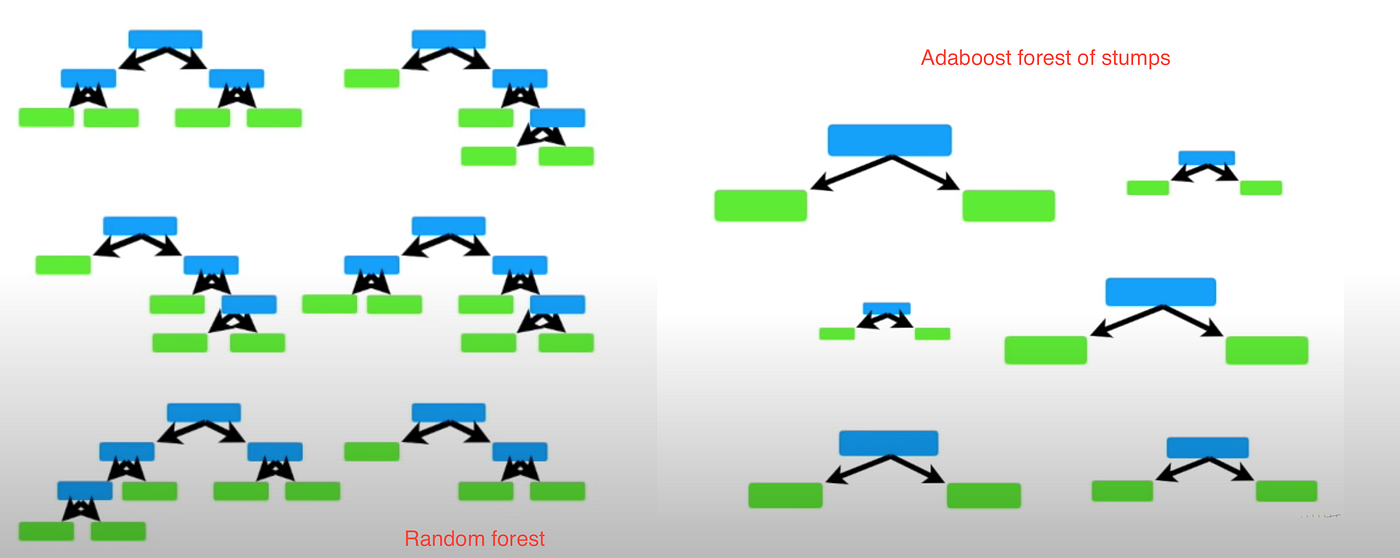
\includegraphics[width=0.7\linewidth]{images/ds_ada.png}
    \caption{Random Forest (nhiều Decision Tree vừa và sâu) vs Ada Boost (nhiều cây nông / Stump)}
\end{figure}
 

\subsection{Ensemble Learning là gì ?}
Thay vì phụ thuộc vào 1 mô  duy nhất,  \textbf{Ensemble Learning} kết hợp nhiều mô hình để cải thiện độ chính xác tổng thể. Ý tưởng cốt lõi là \textit{ý tưởng của nhiều người sẽ tốt hơn ý tưởng của 1 người}.

\begin{figure}[H]
    \centering
    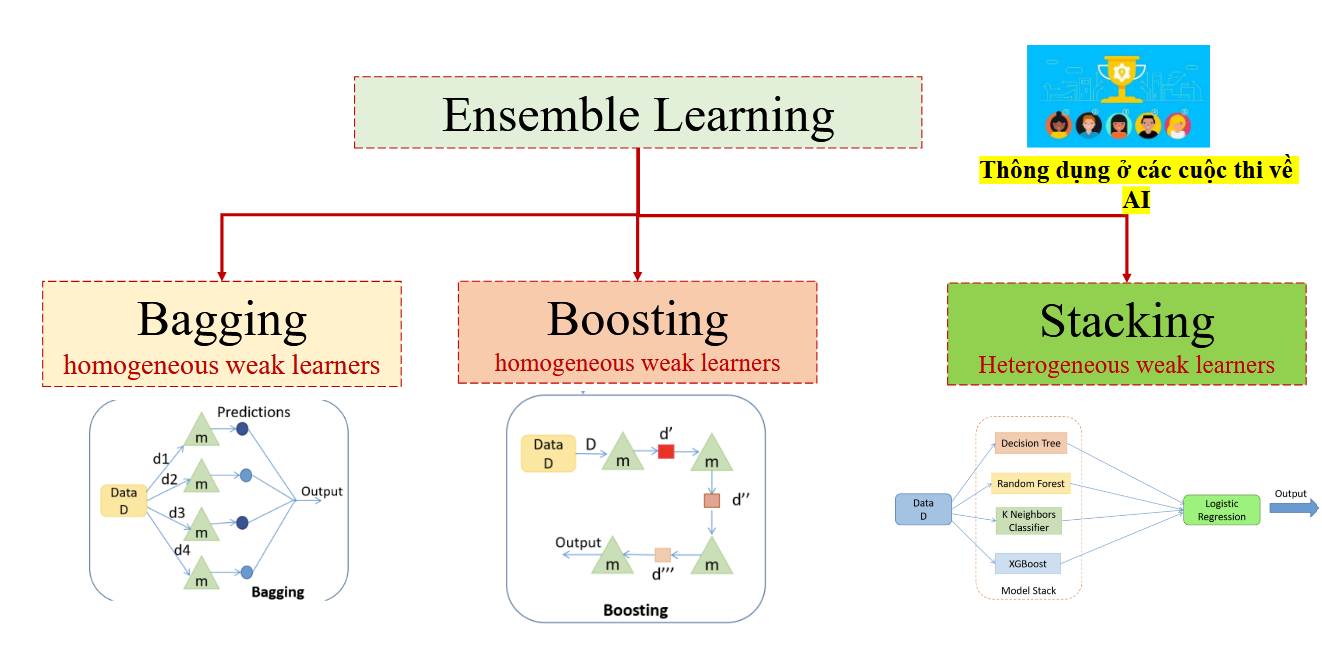
\includegraphics[width=0.7\linewidth]{images/bg_bt_st.png}
    \caption{Essemble Learning}
\end{figure}

\textbf{Bagging} (vd: Random Forest): các mô hình được huấn luyện độc lập và song song trên những tập dữ liệu con (tạo ra bằng bootstrap sampling). Kết quả cuối cùng thường lấy trung bình (đối với bài hồi quy) hoặc bỏ phiếu đa số (đối với bài phân loại). Bagging giúp \textbf{giảm phương sai} vì nó làm “mềm” (soften) đi các quyết định quá nhạy cảm của từng cây riêng lẻ.  

\begin{figure}[H]
    \centering
    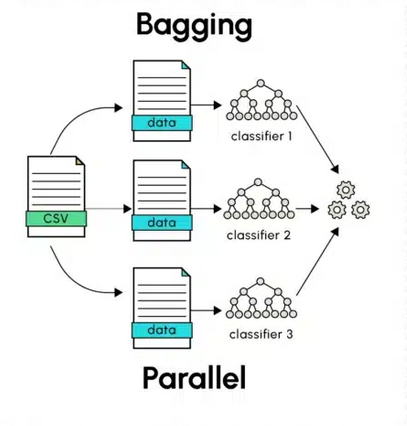
\includegraphics[width=0.4\linewidth]{images/bagging.png}
    \caption{Minh họa quy trình của phương pháp Bagging}
\end{figure}

\textbf{Boosting} (vd AdaBoost, Gradient Boosting): bao gồm các mô hình học tuần tự, mô hình phía sau tập trung giải quyết vấn đề của mô hình phía trước nó để giảm Thiên Vị (bias). AdaBoost bắt đầu từ một mô hình yếu sau đó liên tục bổ sung các mô hình mới tập trung vào những mẫu mà mô hình trước đó dự đoán sai. Qua nhiều vòng lặp, hệ thống dần cải thiện độ chính xác tổng thể.  \\

Ví dụ trực quan: nhiều học sinh “yếu” làm một bài kiểm tra, nhưng nếu mỗi người tập trung vào câu mình giỏi nhất và kết hợp kết quả, thì cả nhóm sẽ làm tốt hơn bất kỳ cá nhân nào.  

\begin{figure}[H]
    \centering
    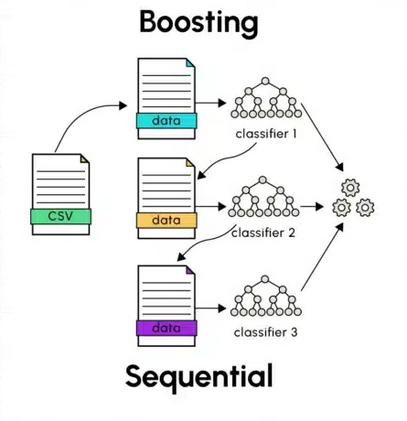
\includegraphics[width=0.4\linewidth]{images/boosting.png}
    \caption{Minh họa quy trình của phương pháp Boosting}
\end{figure}

\textbf{Stacking}: khác với Bagging và Boosting, Stacking không chỉ kết hợp đầu ra của các mô hình cùng loại mà còn có thể sử dụng \textbf{nhiều loại mô hình khác nhau} (Decision Tree, Logistic Regression, Neural Network, …). Đầu ra của các mô hình con sẽ trở thành đặc trưng đầu vào cho một mô hình cuối (gọi là \textit{meta-learner}) để đưa ra dự đoán. Stacking giúp mô hình cuối học cách khai thác \textbf{điểm mạnh bổ sung lẫn nhau} của từng mô hình con.  

\begin{figure}[H]
    \centering
    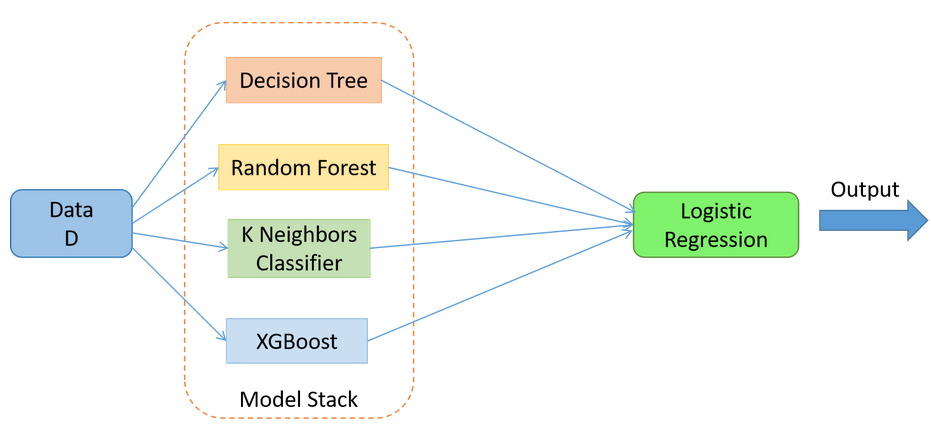
\includegraphics[width=0.7\linewidth]{images/stacking.png}
    \caption{Minh họa quy trình của phương pháp Stacking}
\end{figure}

\textbf{Tóm lại:} Bagging giảm phương sai bằng cách huấn luyện song song và trung bình hóa. Boosting giảm thiên lệch bằng cách học tuần tự và tập trung vào lỗi. Stacking kết hợp nhiều loại mô hình với một meta-learner để khai thác sức mạnh bổ sung của chúng. Đây chính là ba trụ cột quan trọng của Ensemble Learning.

\section{Phần 2: Trực giác đằng sau AdaBoost }
Boosting nói chung có nhiều biến thể, nhưng AdaBoost là một trong những thuật toán đầu tiên và đơn giản nhất.
\begin{figure}[H]
    \centering
    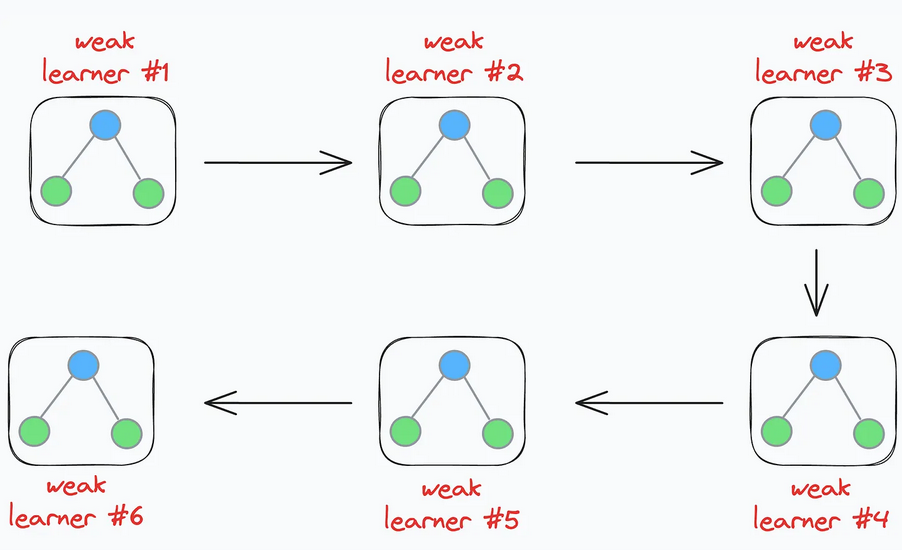
\includegraphics[width=0.7\linewidth]{images/ada_pipeline.png}
    \caption{Minh họa cách AdaBoost hoạt động}
\end{figure}
 Điểm đặc biệt là cách nó phân bổ trọng số cho từng mô hình con 1 cách tuần tự: \textbf{stump nào có dự đoán tốt sẽ có tiếng nói (Amount of say) mạnh trong mô hình cuối cùng.} 
\begin{figure}[H]
    \centering
    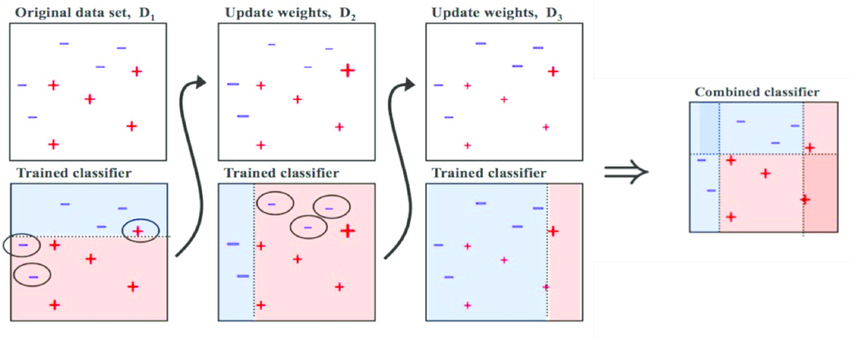
\includegraphics[width=0.85\linewidth]{images/ada_vs.png}
    \caption{Minh họa cách 1 Ada Boost hoàn thiện chia dữ liệu}
\end{figure}


\subsection{Weak Learner là gì ?}
Một DS có độ sâu là 1 gồm 2 lá gọi là Decision Stump và là 1 Weak Learner. Một Stump chỉ xem xét duy nhất 1 đặc trưng để đưa ra quyết định, ví dụ "nếu  \textit{ChestPain} = Có thì dự đoán bệnh tim = Có, ngược lại = Không". Đây là 1 mô hình rất yếu, nhưng khi kết hợp nhiều stump thành AdaBoost nó là một Classifier mạnh mẽ. 

\begin{figure}[H]
    \centering
    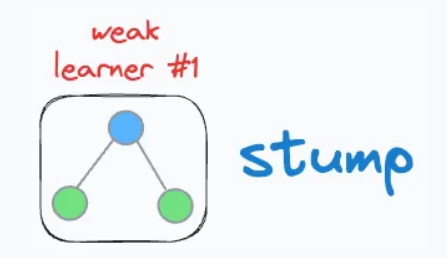
\includegraphics[width=0.3\linewidth]{images/weak.png}
    \caption{Minh họa Weak Learner}
\end{figure}

\subsection{For loop của Ada Boost - Quy trình trực quan}
Mô hình AdaBoost được xây dựng theo một chuỗi các vòng lặp, mỗi bước dùng 1 weak learner (hoặc 1 stump) để cải thiện các lỗi của bước trước. Mình sẽ minh họa quy trình tính toán của Ada Boost 1 cách trực quan trong phần dưới đây:

\begin{enumerate}
  \item \textbf{Khởi tạo trọng số cho tất cả các mẫu:}  
    Ở vòng lặp đầu tiên, ta chưa biết mẫu nào khó hay dễ, nên gán trọng số bằng nhau:  
    \[
    w_i^{(0)} = \frac{1}{n}, \quad i = 1, 2, \ldots, n
    \]  
    Trong đó:  
    \begin{itemize}
        \item \(n\): số lượng mẫu huấn luyện.  
        \item \(w_i^{(0)}\): trọng số của mẫu thứ \(i\) tại vòng lặp 0 (trước khi huấn luyện stump nào).  
    \end{itemize}

    \begin{figure}[H]
    \centering
    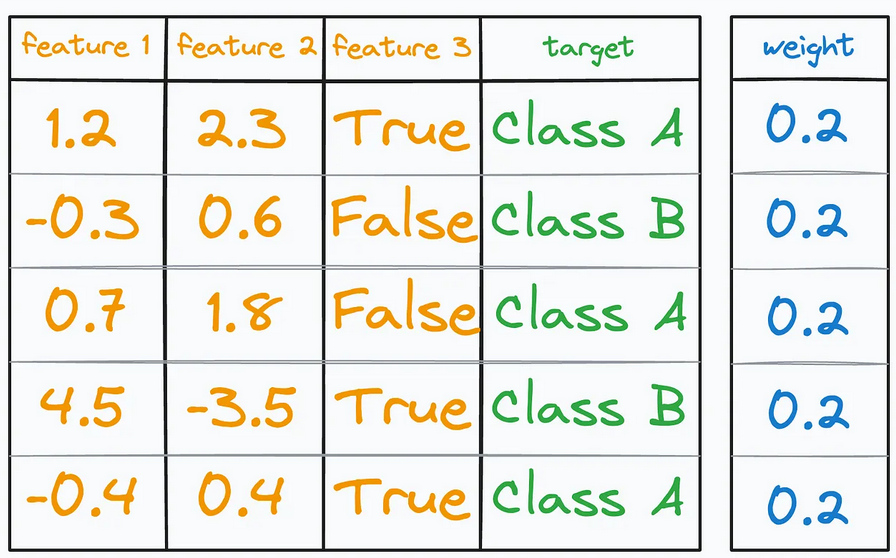
\includegraphics[width=0.7\linewidth]{images/ada_pipeline_2.png}
    \caption{Khởi tạo trọng số đều nhau cho các mẫu}
    \end{figure}
  
  \item \textbf{Huấn luyện stump đầu tiên (weak learner):}  
    Với dữ liệu có trọng số \(w_i^{(0)}\), ta tìm stump \(G_1(x)\) sao cho \textbf{lỗi có trọng số} nhỏ nhất.  
    \begin{itemize}
        \item \(G_1(x)\): dự đoán của stump đầu tiên trên mẫu \(x\).  
        \item Các mẫu có trọng số lớn sẽ ảnh hưởng mạnh hơn đến việc chọn ngưỡng chia của stump.  
    \end{itemize}

    Nếu stump dự đoán 50/50, tức là lỗi \(\varepsilon = 0.5\), thì \(\alpha = 0\) \(\implies\) stump này không mang thêm thông tin, cần bỏ qua hoặc đảo ngược nhãn.

    \begin{figure}[H]
    \centering
    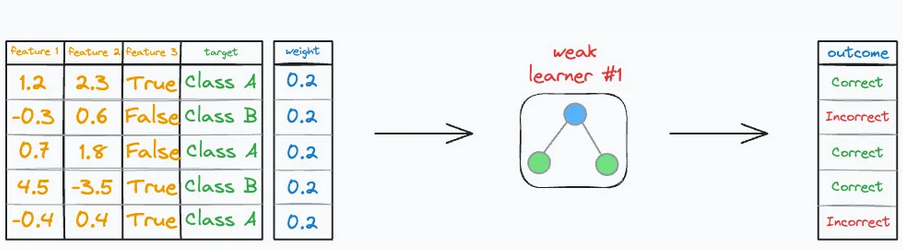
\includegraphics[width=0.7\linewidth]{images/ada_pipeline_3.png}
    \caption{Decision stump đầu tiên được chọn}
    \end{figure}
  
  \item \textbf{Tính lỗi có trọng số của stump:}  
	\textbf{ục tiêu của AdaBoost ở mỗi vòng} là làm sao để stump tiếp theo được đào tạo trên một “phiên bản dữ liệu” mà các mẫu mà mô hình hiện tại dự đoán sai xuất hiện nhiều hơn, để stump mới có cơ hội “sửa” các lỗi đó. \\
          
Để giải quyết vấn đề ở trên ta cần giúp Stump tập trung vào số mẫu sai bằng cách tăng weight của mẫu sai và giảm weight của mẫu lớn trong đó mẫu nào có trọng số lớn mà bị dự đoán sai \(\implies\) stump bị phạt nặng hơn.  \\ 

Để làm thế, ta giữ một bộ trọng số \(w_i\) cho mỗi mẫu; trọng số này quy định tầm quan trọng (và xác suất được chọn trong bootstrap / sampling) khi tạo stump kế tiếp. Mục tiêu là điều chỉnh \(w_i\). sao cho các mẫu sai được tăng trọng số, và các mẫu đúng được giảm hoặc giữ cố định. 

    \[
    \varepsilon_1 = \sum_{i=1}^n w_i^{(0)} \cdot \mathbf{1}\big(y_i \neq G_1(x_i)\big)
    \]  m
    Trong đó: 
    \begin{itemize}
        \item \(y_i\): nhãn thực tế của mẫu \(i\).  
        \item \(G_1(x_i)\): dự đoán của stump đầu tiên.  
        \item \(\mathbf{1}(\cdot)\): hàm chỉ thị, bằng 1 nếu sai, bằng 0 nếu đúng.  
    \end{itemize}
   

  \item \textbf{Tính độ tin cậy, tiếng nói của stump (Amount of Say / $\alpha_1$):}  
    Sức mạnh của stump tỷ lệ nghịch với lỗi của nó:  
    \[
    \alpha_1 = \frac{1}{2} \ln \frac{1 - \varepsilon_1}{\varepsilon_1}
    \]  
    Trong đó:  
    \begin{itemize}
        \item \(\varepsilon_1\): lỗi có trọng số.  
        \item \(\alpha_1\): độ tin cậy của stump.  
    \end{itemize}
    Nếu \(\varepsilon_1 < 0.5\) \(\implies\) stump tốt hơn random \(\implies\) \(\alpha_1 > 0\).  
    Nếu \(\varepsilon_1 = 0.5\) \(\implies\) stump không có giá trị, \(\alpha_1 = 0\).  
    Nếu \(\varepsilon_1 > 0.5\) \(\implies\) stump tệ hơn random, có thể đảo ngược nhãn.

    \begin{figure}[H]
    \centering
    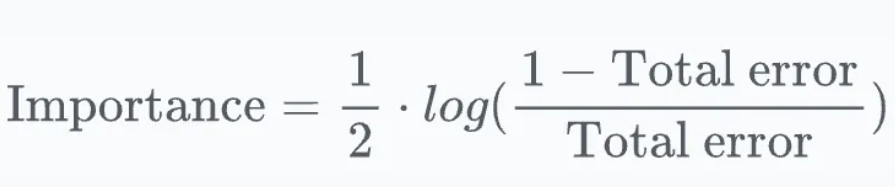
\includegraphics[width=0.7\linewidth]{images/ada_pipeline_for.png}
    \caption{Tính độ tin cậy của stump đầu tiên}
    \end{figure}

  \item \textbf{Cập nhật trọng số mẫu:}  
    Sau khi biết stump nào mạnh, ta cập nhật trọng số để các mẫu khó (dự đoán sai) được chú ý hơn:  
    \[
    w_i^{(1)} = \frac{w_i^{(0)} \cdot \exp\big(-\alpha_1 \, y_i \, G_1(x_i)\big)}{Z_1}
    \]  
    Trong đó:  
    \begin{itemize}
        \item Nếu \(y_i = G_1(x_i)\) (đúng) \(\implies\) \(y_i G_1(x_i) = +1\) \(\implies\) nhân với \(e^{-\alpha_1}\), trọng số giảm.  
        \item Nếu \(y_i \neq G_1(x_i)\) (sai) \(\implies\) \(y_i G_1(x_i) = -1\) \(\implies\) nhân với \(e^{+\alpha_1}\), trọng số tăng.  
        \item \(Z_1\): hằng số chuẩn hóa để \(\sum_i w_i^{(1)} = 1\).  
    \end{itemize}

    Trực giác: \(\alpha_1\) càng lớn \(\implies\) mức phạt/thưởng cho đúng-sai càng mạnh.

    \begin{figure}[H]
    \centering
    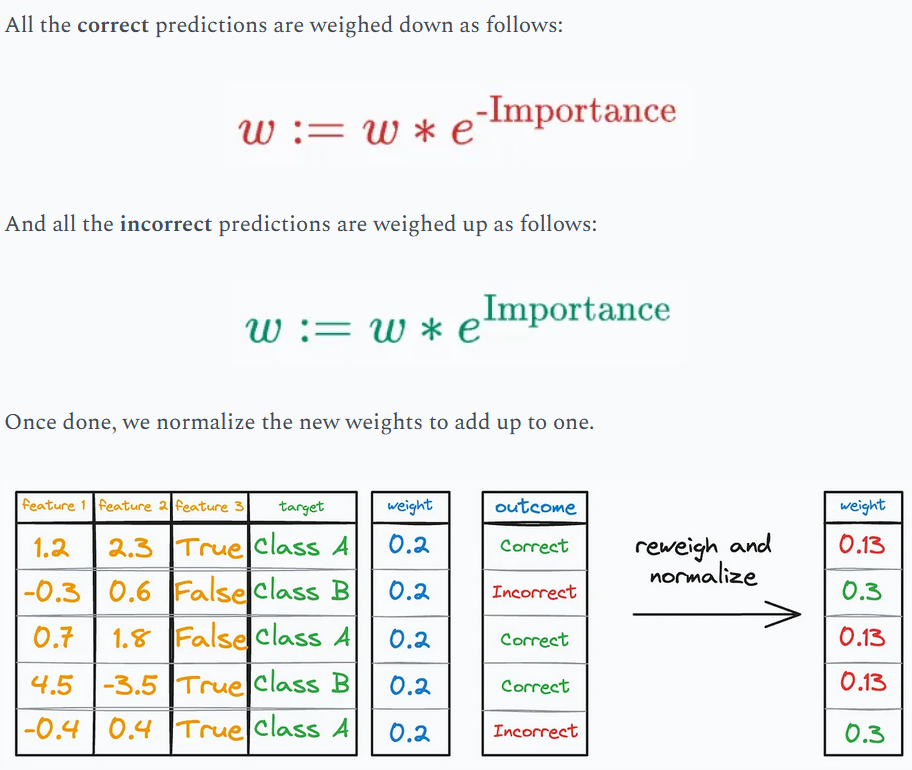
\includegraphics[width=0.7\linewidth]{images/ada_pipeline_6.png}
    \caption{Cập nhật trọng số sau stump đầu tiên}
    \end{figure}

  \item \textbf{Lặp lại các vòng tiếp theo:}  
    Với trọng số mới \(w_i^{(1)}\), ta chọn stump kế tiếp \(G_2(x)\), tính lỗi \(\varepsilon_2\), \(\alpha_2\), rồi lại cập nhật thành \(w_i^{(2)}\).  
    Quá trình này tiếp diễn cho đến khi đạt số vòng \(M\) hoặc mô hình hội tụ.

    \begin{figure}[H]
    \centering
    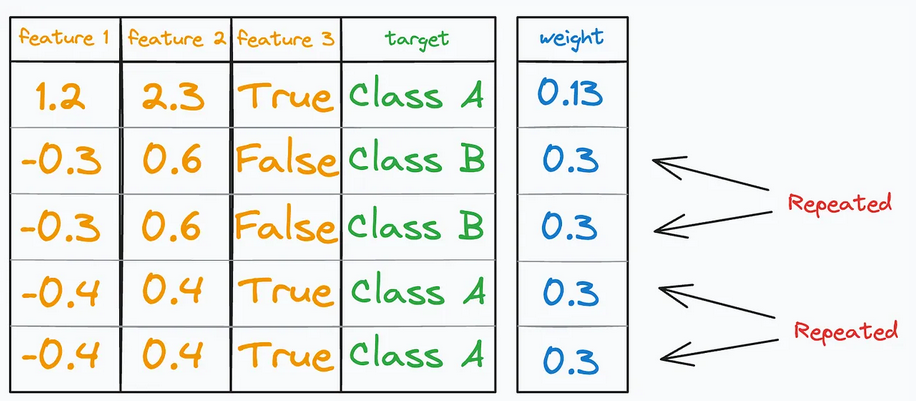
\includegraphics[width=0.7\linewidth]{images/ada_pipeline_7.png}
    \caption{Cập nhật trọng số qua nhiều vòng}
    \end{figure}

  \item \textbf{Kết hợp các stump thành mô hình cuối:}  
    Cuối cùng, AdaBoost kết hợp các stump theo trọng số \(\alpha_m\), để đưa ra tín hiệu kí hiệu là sign() viết tắt cho từ signal:  
    \[
    F(x) = \operatorname{sign}\Big(\sum_{m=1}^M \alpha_m \, G_m(x)\Big)
    \]  
    Trong đó:  
    \begin{itemize}
        \item Stump tốt (có \(\alpha_m\) lớn) \(\implies\) ảnh hưởng mạnh hơn.  
        \item Stump yếu (có \(\alpha_m\) nhỏ) \(\implies\) ảnh hưởng yếu hoặc gần như bị bỏ qua.  
    \end{itemize}

    \begin{figure}[H]
    \centering
    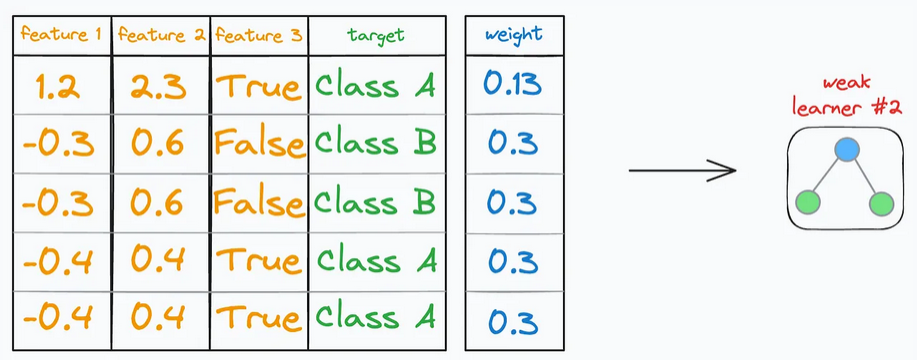
\includegraphics[width=0.7\linewidth]{images/ada_pipeline_8.png}
    \caption{Kết hợp các stump để tạo mô hình AdaBoost cuối cùng}
    \end{figure}
\end{enumerate}


\subsection*{Bảng tổng hợp ký hiệu trong AdaBoost}

\begin{table}[H]
\centering
\begin{tabular}{|c|p{9cm}|}
\hline
\textbf{Ký hiệu} & \textbf{Ý nghĩa và trực giác} \\
\hline
\(x_i\) & Mẫu dữ liệu huấn luyện thứ \(i\). \\
\hline
\(y_i \in \{-1, +1\}\) & Nhãn thực tế của mẫu \(i\) (dùng \(-1, +1\) thay vì \(0,1\) để tiện cho công thức nhân). \\
\hline
\(w_i^{(m)}\) & Trọng số của mẫu \(i\) tại \textbf{vòng lặp \(m\)}.  
- \(^{(0)}\): trước khi huấn luyện bất kỳ stump nào (khởi tạo bằng \(1/n\)).  
- \(^{(1)}\): sau khi huấn luyện stump đầu tiên và cập nhật trọng số.  
- Tương tự cho các vòng tiếp theo. \\
\hline
\(G_m(x)\) & Weak learner (thường là Decision Stump) được huấn luyện tại vòng \(m\). Đây là một hàm phân loại trả về \(-1\) hoặc \(+1\). \\
\hline
\(\varepsilon_m\) & Lỗi có trọng số của stump với ký hiệu là epsilon thứ \(m\):  
\(\varepsilon_m = \sum_i w_i^{(m-1)} \cdot \mathbf{1}(y_i \neq G_m(x_i))\).  
Nếu stump sai nhiều trên các mẫu quan trọng, \(\varepsilon_m\) sẽ cao. \\
\hline
\(\alpha_m\) & Độ tin cậy (\textit{amount of say}) của stump thứ \(m\):  
\(\alpha_m = \tfrac{1}{2} \ln \tfrac{1 - \varepsilon_m}{\varepsilon_m}\).  
Stump càng chính xác thì \(\alpha_m\) càng lớn $\implies$ có ảnh hưởng nhiều hơn trong kết quả cuối. \\
\hline
\(Z_m\) & Hằng số chuẩn hóa tại vòng \(m\), đảm bảo \(\sum_i w_i^{(m)} = 1\). \\
\hline
\(F(x)\) & Mô hình AdaBoost cuối cùng:  
\(F(x) = \operatorname{sign}\big(\sum_{m=1}^M \alpha_m G_m(x)\big)\).  
Dự đoán được đưa ra dựa trên “phiếu bầu có trọng số” của các stump. \\
\hline
\end{tabular}
\end{table}


\section{Phần 3: Công thức toán đằng sau AdaBoost}
    \begin{figure}[H]
    \centering
    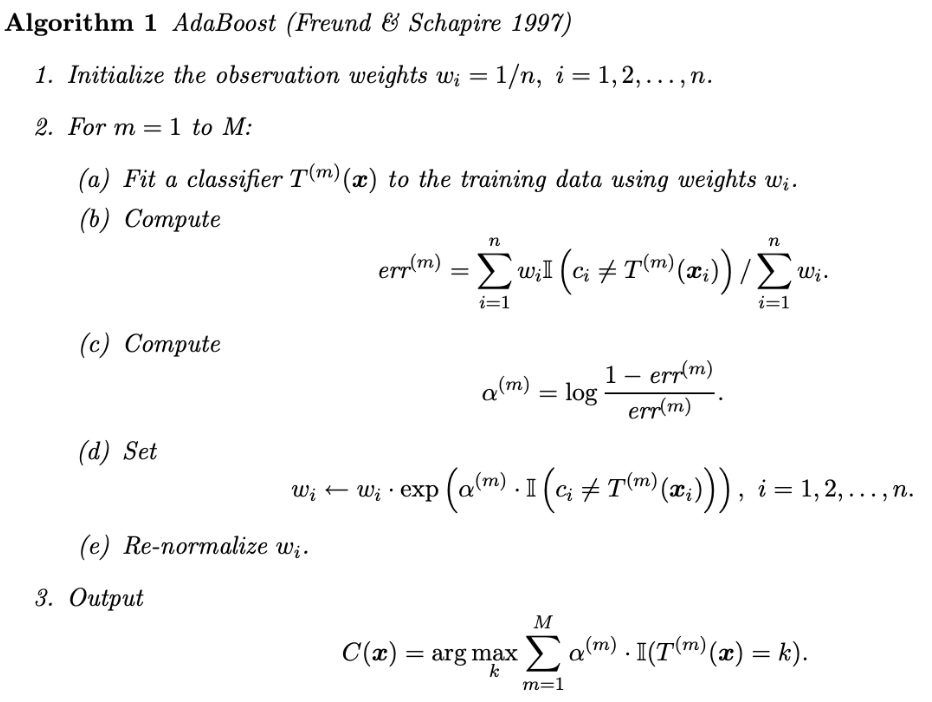
\includegraphics[width=0.7\linewidth]{images/math_ada_1.png}
    \caption{Thuật toán gốc của Ada Boost}
    \end{figure}
Thuật toán AdaBoost được xây dựng trên một vòng lặp “học – sửa sai – học lại”, thuật toán nói rằng mỗi vòng chọn ra một \textit{weak learner} (Stump) mới để sửa chữa thất bại của stump trước.  
\begin{itemize}
    \item Khi bắt đầu, tất cả các mẫu dữ liệu có trọng số bằng nhau, tức là ta coi chúng quan trọng như nhau.
    \item For Loop: huấn luyện một stump dựa trên trọng số hiện tại. Sau đó kiểm tra nó sai ở đâu.
    \item Nếu stump sai trên mẫu nào \(\implies\) mẫu đó được flag (đánh dấu, báo hiệu) là 1 và trọng số tăng lên để lần sau mô hình quan tâm nhiều hơn.
    \item Ngược lại, mẫu đúng thì được giảm trọng số (ít quan trọng hơn ở vòng sau).
    \item Lặp lại quy trình trên nhiều vòng, cuối cùng kết hợp các stump bằng cách bỏ phiếu có trọng số.
\end{itemize}


\subsection*{2. Hàm giả thuyết (Hypothesis Function)}

    \begin{figure}[H]
    \centering
    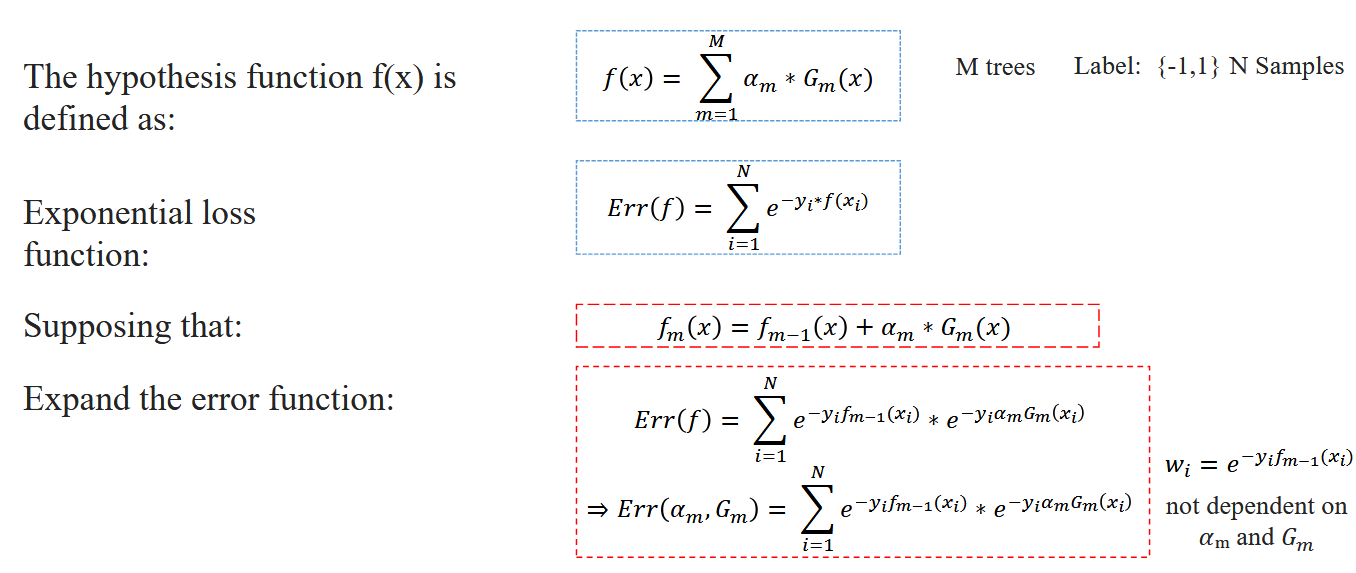
\includegraphics[width=0.7\linewidth]{images/math3.png}
    \end{figure}


Công thức được tạo ra với ý tưởng là quyết định cuối cùng sẽ được quyết định bở đóng góp của mỗi stump, nói cách khác là tổng các stump có trọng số:
\[
f(x) = \sum_{m=1}^M \alpha_m G_m(x)
\]

\begin{itemize}
    \item \(M\): số vòng lặp (số stump).
    \item \(G_m(x)\): weak learner thứ \(m\).
    \item \(\alpha_m\): độ tin cậy (amount of say) của stump thứ \(m\).
\end{itemize}

\textbf{Vai trò:} công thức này định nghĩa AdaBoost như một mô hình tuyến tính trong không gian của các stump. Kết quả dự đoán cuối cùng là dấu của \(f(x)\).



\subsection*{3. Hàm mất mát mũ (Exponential Loss)}

    \begin{figure}[H]
    \centering
    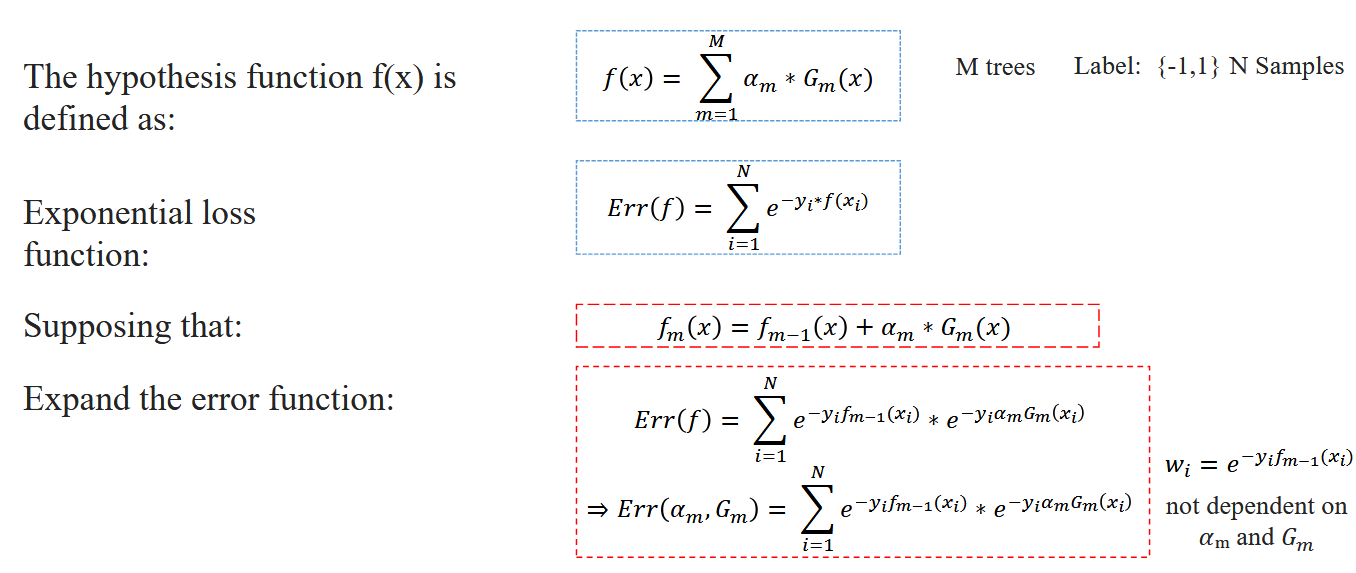
\includegraphics[width=0.7\linewidth]{images/math3.png}
    \end{figure}
Để học ra được \(\alpha_m\), AdaBoost không chọn ngẫu nhiên mà tối ưu một hàm mất mát:
\[
Err(f) = \sum_{i=1}^N e^{-y_i f(x_i)}
\]

\begin{itemize}
    \item \(y_i \in \{-1, +1\}\): nhãn thật.  
    \item Nếu \(y_i f(x_i)\) lớn dương \(\implies\) mẫu dự đoán đúng và tự tin, mất mát gần 0.  
    \item Nếu \(y_i f(x_i)\) âm \(\implies\) mẫu sai, mất mát tăng rất nhanh (vì số mũ).
\end{itemize}

\textbf{Liên hệ:} giống như trong \textit{logistic regression}, ta cũng dùng hàm mất mát có log/exp (vd: cross-entropy) để phạt nặng các dự đoán sai. Ở AdaBoost, exponential loss đảm bảo “mẫu sai càng nặng thì càng được chú ý”. Ada Boost khá là giống Neural network khi mỗi node đều được tính loss và node sau cải thiện node trước nó.


\subsection*{4. Mở rộng tại vòng lặp thứ $m$}

    \begin{figure}[H]
    \centering
    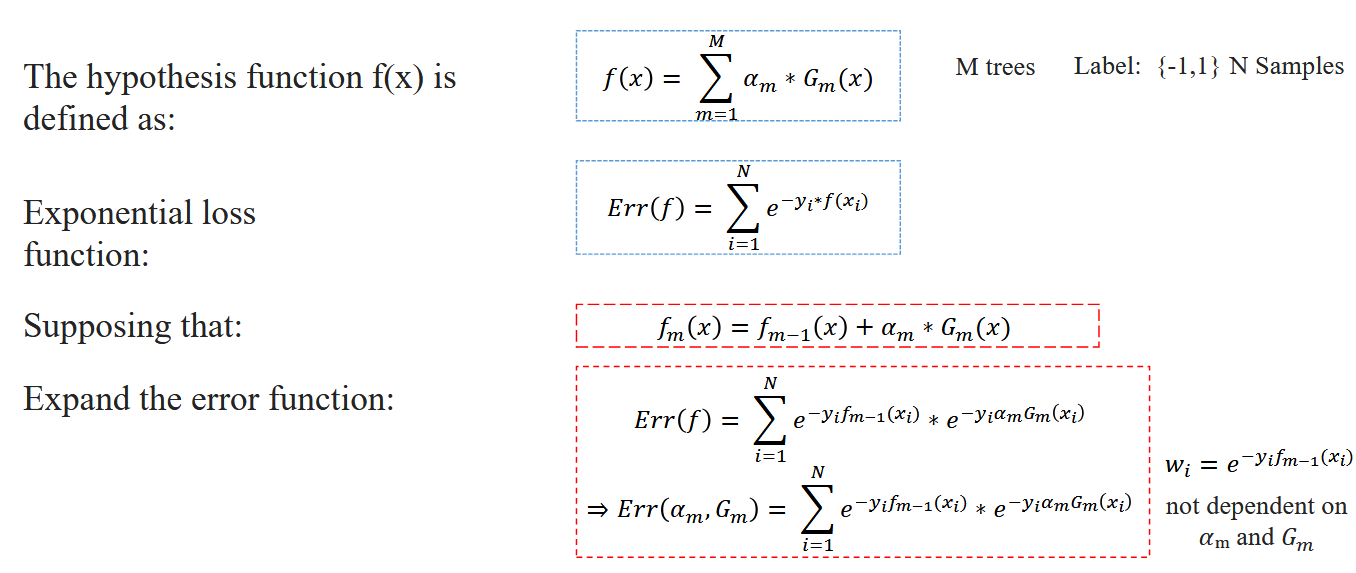
\includegraphics[width=0.7\linewidth]{images/math3.png}
    \end{figure}


Ở vòng \(m\), mô hình được viết thành:
\[
f_m(x) = f_{m-1}(x) + \alpha_m G_m(x)
\]

Thay vào hàm mất mát:
\[
Err(f) = \sum_{i=1}^N e^{-y_i f_{m-1}(x_i)} \cdot e^{-y_i \alpha_m G_m(x_i)}
\]

Đặt:
\[
w_i = e^{-y_i f_{m-1}(x_i)}
\]

\textbf{Ý nghĩa:} \(w_i\) chính là trọng số hiện tại của mẫu \(i\). Nó không phụ thuộc vào \(\alpha_m\) hay \(G_m\), mà phản ánh mức độ khó/dễ của mẫu tính tới vòng \(m-1\).


\subsection*{5. Tách thành mẫu đúng và sai}

    \begin{figure}[H]
    \centering
    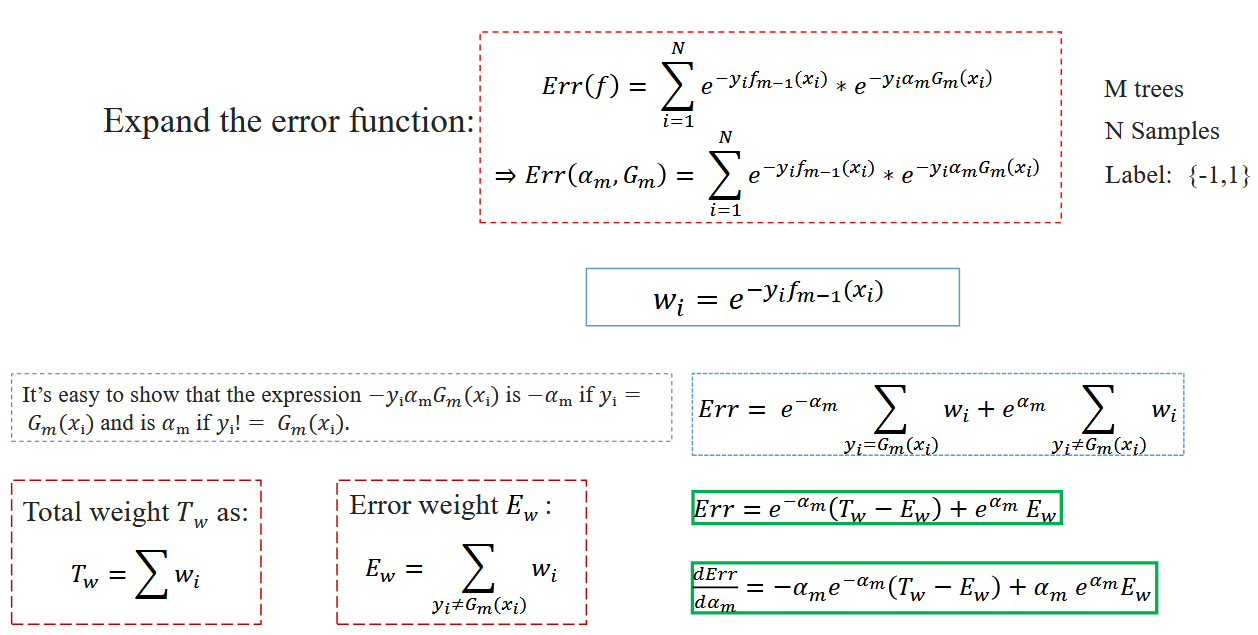
\includegraphics[width=0.7\linewidth]{images/math4.png}
    \end{figure}

Ta gom các mẫu theo việc stump dự đoán đúng hay sai:
\[
Err(\alpha_m, G_m) = e^{-\alpha_m} \sum_{y_i = G_m(x_i)} w_i \;+\; e^{+\alpha_m} \sum_{y_i \neq G_m(x_i)} w_i
\]

\begin{itemize}
    \item Mẫu đúng: bị nhân với \(e^{-\alpha_m}\) (giảm trọng số).  
    \item Mẫu sai: bị nhân với \(e^{+\alpha_m}\) (tăng trọng số).  \\
\end{itemize}

\noindent Đặt tổng trọng số là:
\[
T_w = \sum_i w_i, \quad 
\]
và tổng trọng số của mẫu dự đoán sai là:
\[
E_w = \sum_{y_i \neq G_m(x_i)} w_i
\] trong đó \(y_i \neq G_m(x_i)\) nghĩa là nhãn thực tế \(y_i\) của stump thứ i khác nhãn dự đoán \(G_m(x) \)


Ta có :
\[
Err(\alpha_m) = e^{-\alpha_m}(T_w - E_w) + e^{+\alpha_m} E_w
\]



\subsection*{6. Tối ưu $\alpha_m$ bằng đạo hàm}
    \begin{figure}[H]
    \centering
    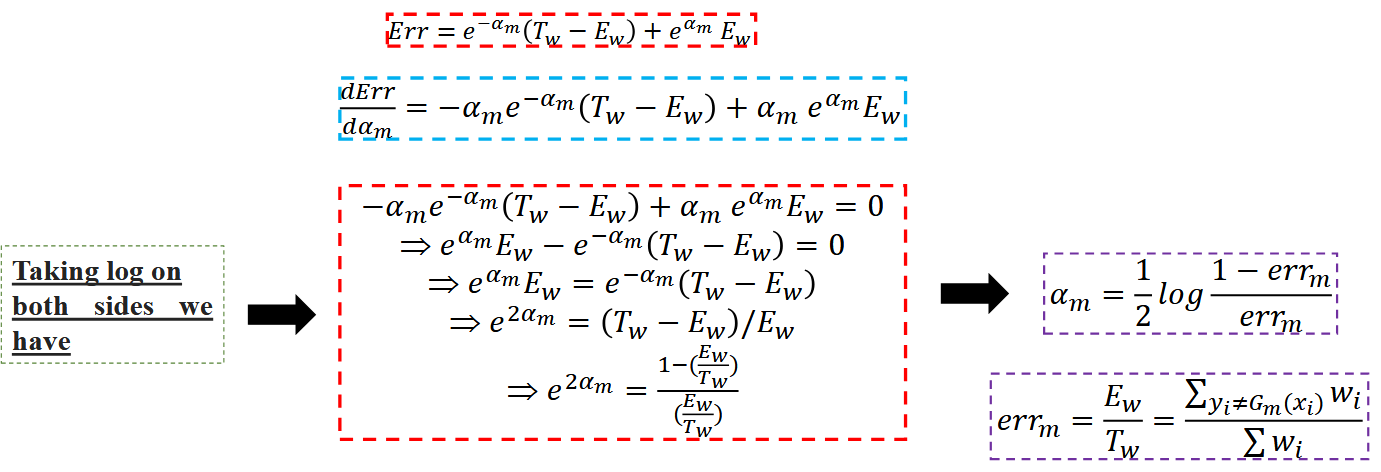
\includegraphics[width=0.7\linewidth]{images/math5.png}
    \caption{Tính cực tiểu của hàm mất mát}
    \end{figure}

Để chọn \(\alpha_m\) tối ưu, ta lấy đạo hàm (vì đạo hàm giúp tìm ra hàm để tối thiểu error và mình đang cần 1 hàm để tối thiểu error):
\[
\frac{dErr}{d\alpha_m} = -e^{-\alpha_m}(T_w - E_w) + e^{+\alpha_m} E_w
\]

Đặt hàm bằng 0 để tối ưu:
\[
e^{2\alpha_m} = \frac{T_w - E_w}{E_w}
\]

Suy ra:
\[
\alpha_m = \frac{1}{2} \ln \frac{T_w - E_w}{E_w}
\]

Mà \(\frac{E_w}{T_w} = err_m\), lỗi có trọng số tại for loop \(m\).

Do đó:
\[
\alpha_m = \frac{1}{2} \ln \frac{1 - err_m}{err_m}
\]

\textbf{Ý tưởng đằng sau là:} nếu stump tốt (err nhỏ), \(\alpha_m\) lớn \(\implies\) stump có tiếng nói mạnh. Nếu stump chỉ đoán ngẫu nhiên (err = 0.5) \(\implies\) \(\alpha_m = 0\), không đóng góp.


\subsection*{7. tóm tắt lại Thuật toán AdaBoost}

Kết nối lại với Algorithm 1:
\begin{enumerate}
    \item Bắt đầu với trọng số đều nhau.  
    \item Ở mỗi vòng: huấn luyện stump \(G_m\) dựa trên trọng số hiện tại.  
    \item Tính lỗi có trọng số \(err_m\).  
    \item Tính độ tin cậy \(\alpha_m\).  
    \item Cập nhật trọng số: mẫu sai tăng, mẫu đúng giảm.  
    \item Chuẩn hóa trọng số để tổng = 1.  
\end{enumerate}

Ta được mô hình cuối cùng là:
\[
F(x) = \operatorname{sign}\Big(\sum_{m=1}^M \alpha_m G_m(x)\Big)
\]


\subsection{Ada Boost cho bài toán đa lớp:} Ở trên ta đã biết thuật toán AdaBoost gốc cho bài toán phân loại nhị phân (binary classification), còn thuật toán SAMME là một phiên bản mở rộng của AdaBoost cho bài toán phân loại đa lớp (multi-class classification). Tổng quan công thức giống y chang AdaBoost gốc nhưng thêm 1 tham số K, vậy K là gì và nó làm được gì ?

\begin{figure}[H]
    \centering
    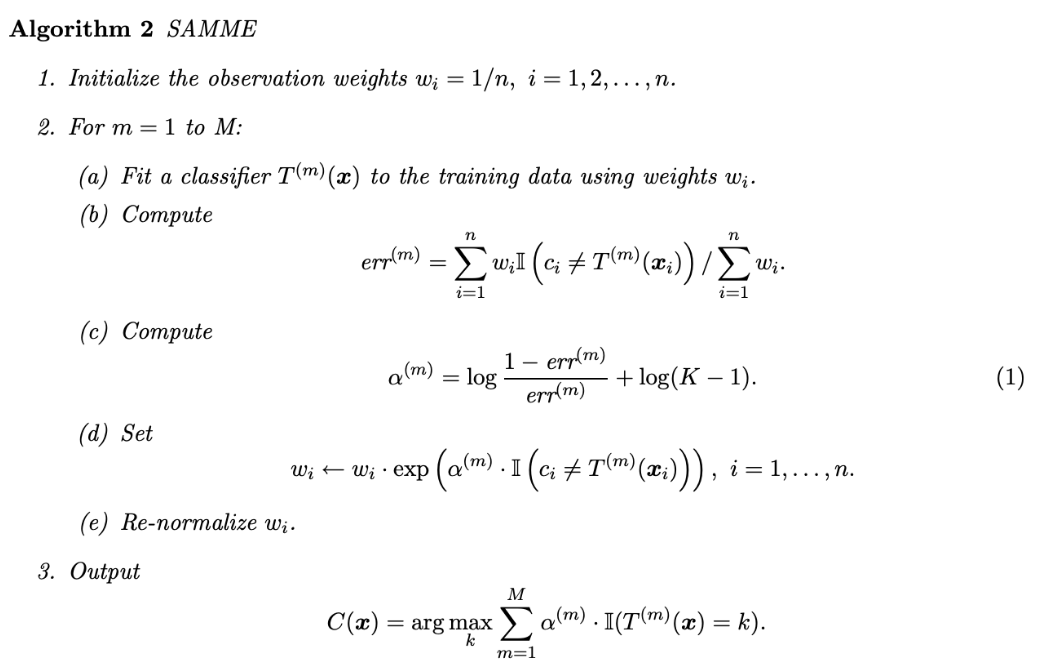
\includegraphics[width=0.7\linewidth]{images/math_ada_2.png}
    \caption{SAMME (Stagewise Additive Modeling using a Multiclass Exponential loss function) cho bài toán phân loại đa lớp}
\end{figure}

\begin{itemize}
    \item \textbf{Phân loại nhị phân (AdaBoost):}
    Công thức cập nhật trọng số $\alpha^{(m)}$ chỉ bao gồm một phần, được chứng minh từ việc tối thiểu hóa hàm mất mát cho hai lớp.
    \[
    \alpha^{(m)} = \frac{1}{2} \log \frac{1 - err^{(m)}}{err^{(m)}}
    \]

    \item \textbf{Phân loại đa lớp (SAMME):}
    Công thức cập nhật trọng số $\alpha^{(m)}$ được bổ sung một số hạng phụ thuộc vào số lớp $K$, giúp điều chỉnh độ lớn của $\alpha^{(m)}$ cho bài toán phức tạp hơn.
    \[
    \alpha^{(m)} = \log \frac{1 - err^{(m)}}{err^{(m)}} + \log(K - 1)
    \]
\end{itemize}

\noindent \textbf{Giải thích các thành phần của công thức SAMME:}
\begin{itemize}
    \item Phần đầu tiên $\log\frac{1 - err^{(m)}}{err^{(m)}}$ tương tự như AdaBoost nhưng không có hệ số $\frac{1}{2}$, được gọi là \textbf{trọng số log-odd}. Nó phản ánh độ "tốt" của bộ phân loại yếu thông qua tỉ lệ giữa dự đoán đúng và sai.
\[
\text{Odds} = \frac{\text{P}}{\text{1 - P}}
\]

\[
\text{Log-odds} = \log\left(\frac{\text{P}}{\text{1 - P}}\right) 
= \log\left(\frac{\text{1 - (1 - P)}}{\text{1 - P}}\right) 
= \log\left(\frac{\text{1 - err}}{\text{err}}\right)
\]


    \item Phần thứ hai $+\log(K - 1)$ là phần bổ sung quan trọng nhất. Nó được thêm vào để điều chỉnh trọng số cho bài toán đa lớp, đảm bảo rằng ngay cả khi một bộ phân loại yếu có lỗi $err^{(m)}$ cao hơn $0.5$, trọng số $\alpha^{(m)}$ vẫn có thể dương, giúp mô hình học được.
\end{itemize}

\noindent \textbf{K} đại diện cho số lượng lớp. Vai trò của nó là điều chỉnh độ lớn của $\alpha$ để đảm bảo mỗi bộ phân loại yếu đóng góp đủ "tiếng nói" trong bài toán phân loại đa lớp, giúp thuật toán hội tụ hiệu quả hơn.

\printbibliography
\end{document}
